\documentclass{article}
\usepackage[utf8]{inputenc}
\usepackage[slovene]{babel}
\usepackage{graphicx}

\title{Naloga 2}
\author{William Brooks}
\date{04.04.2020}

\begin{document}

\maketitle

\begin{figure}[h]
\begin{center}

    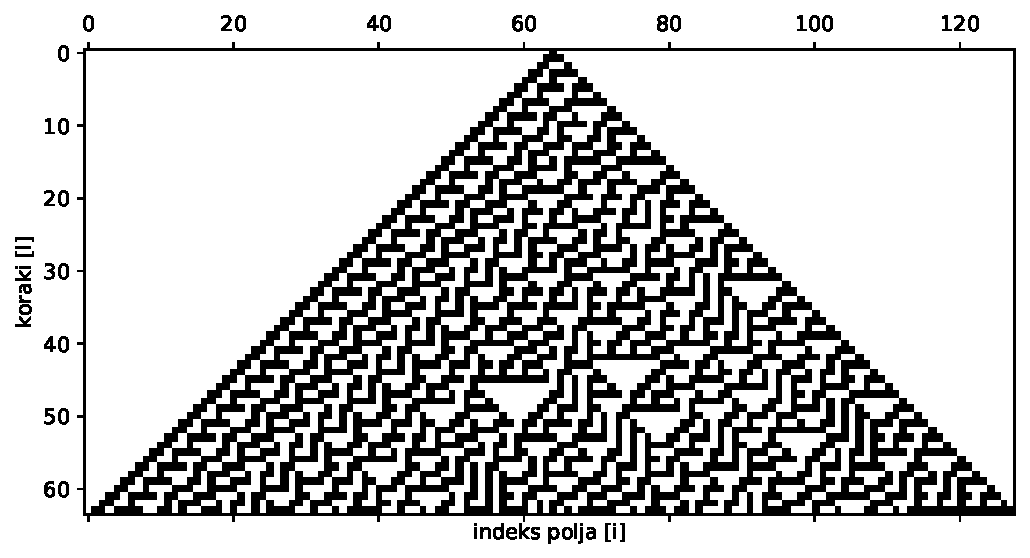
\includegraphics[width=9.5cm]{mat.pdf}
\caption{Prikaz prvih 64 korakov celi\v cnega avtomata.}

\end{center}
\end{figure}

\begin{figure}[h]
\begin{center}

    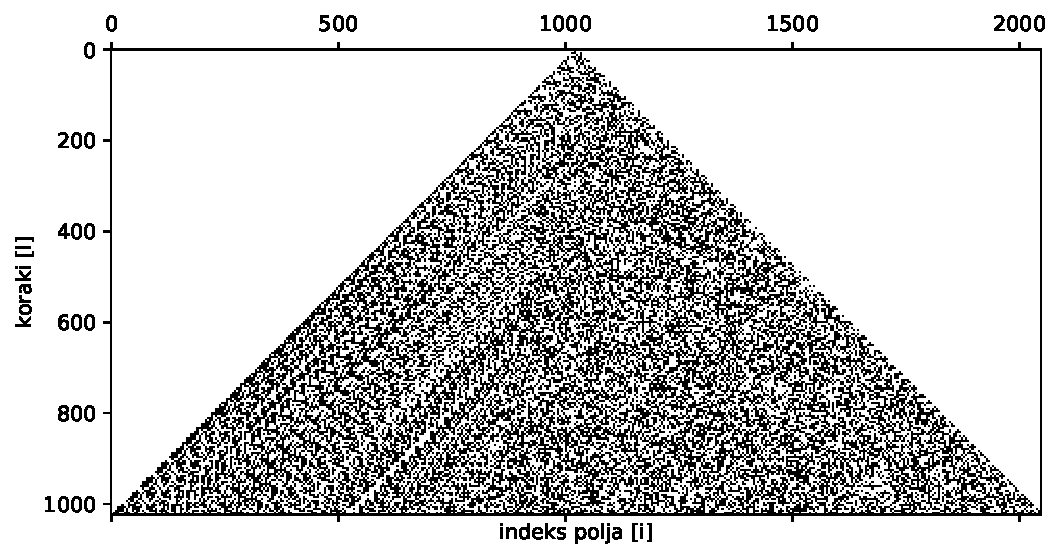
\includegraphics[width=9.5cm]{mat2.pdf}
\caption{Prikaz prvih 1024 korakov avtomata.}

\end{center}
\end{figure}

\begin{figure}[h]
\begin{center}

    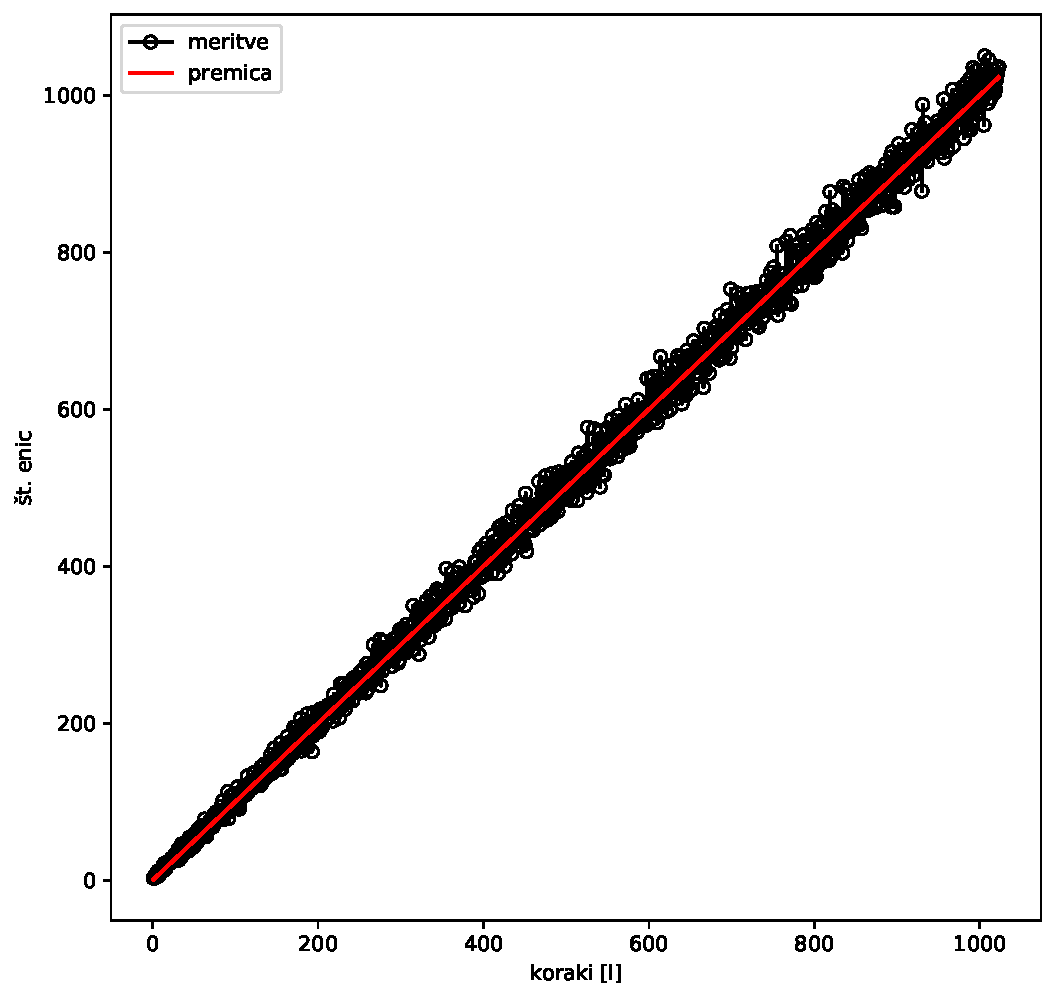
\includegraphics[width=12cm]{vsota.pdf}
\caption{Graf prika\v ze vsoto nepraznih bitov v vsaki vrstici (ozna\v ceni s \v crnimi krogi) v primerjavi s premico skozi izhodi\v s \v ce.}

\end{center}
\end{figure}

\begin{figure}[h]
\begin{center}

    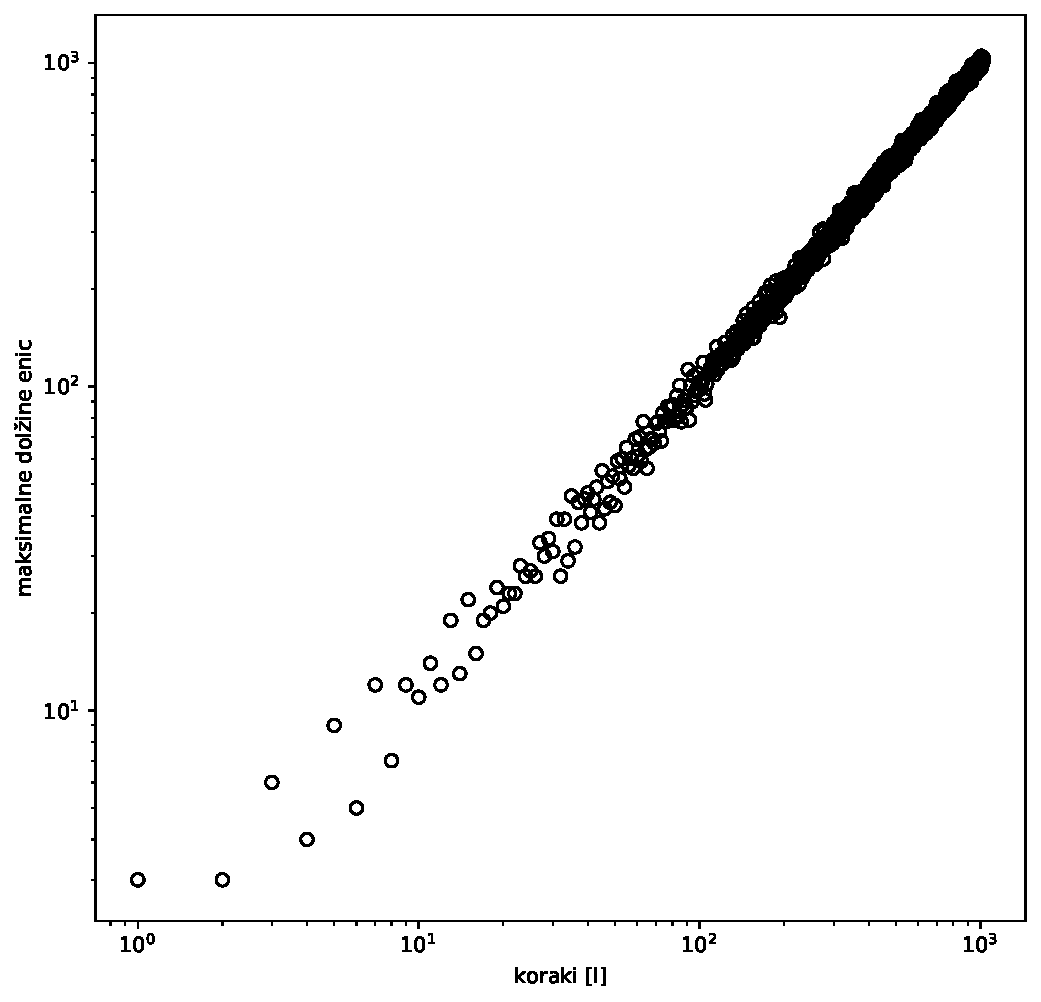
\includegraphics[width=12cm]{skupki.pdf}
\caption{Zadnji graf prika\v ze sepremembo maksimalne dol\v zine nepraznih bitov, ki jih najdemo v posameznem stanju, na logaritmi\v cni skali.}

\end{center}
\end{figure}

\end{document}
